%\documentclass[10pt,a4paper]{article}
\documentclass[letterpaper,10pt,draftclsnofoot,onecolumn]{article}
\usepackage[letterpaper, margin=.75in]{geometry}

\usepackage{hyperref}
\usepackage{listings}
\usepackage{wasysym}
\usepackage{graphicx}

\hypersetup{
	colorlinks,
	citecolor=black,
	filecolor=black,
	linkcolor=black,
	urlcolor=black
}

\begin{document}
\begin{titlepage}
\vspace*{\fill}
\begin{center}
{\Large Tut-Tut, The IoT Rain Fall Detector Design Document}
\\[0.3cm]

{\large Team 21}
\\[0.3cm]

{\large CS 461 - Fall 2018}
\\[0.3cm]

{\large Michael Gillett, Casing and Microcontroller Lead}
\\[0.3cm]
{\large Jonathan Rohr, Data Collection and Management Lead}
\\[0.3cm]
{\large Shreyans Khunteta, UI Lead}
\\[0.3cm]

{\large November 26, 2018}
\\[1cm]

{\Large \textbf{Abstract}}
\end{center}
 Tut-Tut, the IoT Raindrop Detector, is a project under the domain of the OPEnS (Openly Published Environment Sensing) Lab at Oregon State University. Tut-Tut will be able to detect a drop of any size, get an idea of the raindrop mass from the intensity at which it falls, and detect the frequency of raindrops. After Tut-Tut gathers this data, it will be able to wirelessly transmit the information to a central server and communicate it to other IoT devices around Oregon State University. The detector will wake up with a single raindrop and will stay awake as long as rain is detected within a minute. If it does not detect raindrops within a minute, it will go back to sleep. In addition to the physical device, we will also design an online mobile application to which the physical device will transmit information about the raindrops.
\vspace*{\fill}
\end{titlepage}

\section{Introduction}
This document will go into depth on the progress made in Fall Term regarding our project. Our device is known as Tut-Tut, the IoT (Internet of Things) Rainfall Detector, and will serve the OPEnS Lab's ecosystem of environmental sensing devices which they call Loom. Tut-Tut will measure the rainfall by reading the mechanical stress of drops hitting its built-in sensor, and relay it to their server using PushingBox technology. The metrics Tut-Tut wants to know are how hard the drops hit the device, and how often a rain drop strikes it. These values will be continually updated into an easily accessible spreadsheet. In the document, we will linearly outline all of our progress so far, discuss all the problems encountered this term, include any plans we have to fix those problems next term in a retrospective table.

\section{Current Progress \& Problems}
This term we began work on Tut-Tut in week four, when we were assigned the project. We met with Professor Chet Udell that week and were given an Adafruit Feather M0 microcontroller to work with. Professor Udell told us to have a blinking microcontroller by the next week. We were unable to run any Arduino sketches on our microcontroller and thought initially that it was a problem with our drivers, as it wasn't working on any of our computers. We had a wide range of laptops and operating systems between us, so that was baffling. We brought it into the OPEnS Lab and the staff discovered the microcontroller we had been given was faulty. We exchanged it for a new one that worked much better and were able to show the microcontroller blinking to Professor Udell and the OPEnS staff minutes after being given an operational microcontroller.
\\
\\
After this, we were told the names of the sensors and transducers we had to acquire. We were able to order them online and have them delivered to Michael Gillett's Corvallis home. However, Michael was in a horrific car accident on his way to Portland the weekend before Thanksgiving and was stranded there for 8 days. We were unable to open his mailbox and get our equipment, so that delayed us by a week and a half.
\\
\\
We've also had some difficulty in being able to meet with Professor Udell due to his busy schedule. We have a set meeting time on Thursdays, but because we started this project midway through the term and because some meetings have to be cancelled abruptly due to Professor Udell's busy schedule, we haven't had as much time with him as we would like.
\\
\\
However, we were able to produce a Problem Statement, Requirements document, three detailed Tech Reviews, a Design Document and weekly progress reports since week four. This will help us in setting goals and guidelines for the assignment going forward. 
\\
\\
The Problem Statement was used to develop a working definition of the problem we're solving. Normal rainfall collectors do not provide enough information for the needs of the OPEnS Lab. Our client wants a small, portable, disc-shaped device that can detect and provide detailed information about falling rain in real-time. Information includes rainfall rate, intensity, and density. We also defined Tut-Tut's eventual goals and use cases for them.
\\
\\
The Requirements document was used to define Tut-Tut's scope and our eventual goals for it. This was the "What" document that we used to explain our target audience, our project scope, our business case, user characteristics, assumptions/dependencies and our constraints. The system will be a 2x2 inch waterproof sensor capable of detecting even the most minute amounts of rain. It will have wi-fi or network capabilities and we will be able to integrate it easily with the IoT mesh network around the university. It will be able to detect the size of a raindrop, the frequency at which rain is falling, and the intensity at which it hits the detector.
\\
\\
During the Tech Review, each of us submitted an individual tech review for technologies we are taking responsibility for: data collection and management, microcontroller and 3D printed shell, and coding tools. During these documents we identified the tools we would need to accomplish the task ahead of us, and we explored different alternative methods to implement these different technologies. For example, when listing different usable technologies for the Shell, Michael listed three different potential technologies - Inventor, Onshape and AutoCAD. After exploring each in detail, he explained why we would be using AutoCAD ultimately.
\\
\\
Finally, we wrote the Design Document. In the Design document we described our timeline and explained the design of our project in all respects - the Code Design, the Casing Design, our Data Design (how we would collect and manage data), and our Human Interface Design.  We drew upon our previous Tech Review and Requirements documents to properly write this Design Document.


\section{Pieces of code}
\begin{lstlisting}[language=C]
/*
  Knock Sensor

  This sketch reads a piezo element to detect a knocking sound.
  It reads an analog pin and compares the result to a set threshold.
  If the result is greater than the threshold, it writes "knock" to the serial
  port, and toggles the LED on pin 13.

  This example code is in the public domain.

  http://www.arduino.cc/en/Tutorial/Knock
*/


// these constants won't change:
const int ledPin = 13;      // LED connected to digital pin 13
const int knockSensor = A0; // the piezo is connected to analog pin 0
const int threshold = 100;  // threshold value to decide when the detected sound is a knock or not


// these variables will change:
int sensorReading = 0;      // variable to store the value read from the sensor pin
int ledState = LOW;         // variable used to store the last LED status, to toggle the light
\\
void setup() {\\
  pinMode(ledPin, OUTPUT); // declare the ledPin as as OUTPUT
  Serial.begin(9600);       // use the serial port
}

void loop() {
  // read the sensor and store it in the variable sensorReading:
  sensorReading = analogRead(knockSensor);

  // if the sensor reading is greater than the threshold:
  if (sensorReading >= threshold) {
    // toggle the status of the ledPin:
    ledState = !ledState;
    // update the LED pin itself:
    digitalWrite(ledPin, ledState);
    // send the string "Knock!" back to the computer, followed by newline
    Serial.println("Knock!");
  }
  delay(100);  // delay to avoid overloading the serial port buffer
}
\end{lstlisting}

Because of the fact that we have not been able to test our sensors, we have not written any code for the microcontroller yet. We plan to use this example as a basis for Tut-Tut. The "knock" will be drops of water on the piezoelectric sensor, and the Serial.println function will be the PushingBox API uploading the data to our central server. We also have received a code example using interrupts which could prove useful in letting Tut-Tut sleep when no rain is falling. By having a drop generate an interrupt to wake up the device instead of constantly being active, we could save battery.

\section*{Basic Sketch}
\begin{center}
Figure 1: A basic drawing of what Tut-Tut will resemble when complete
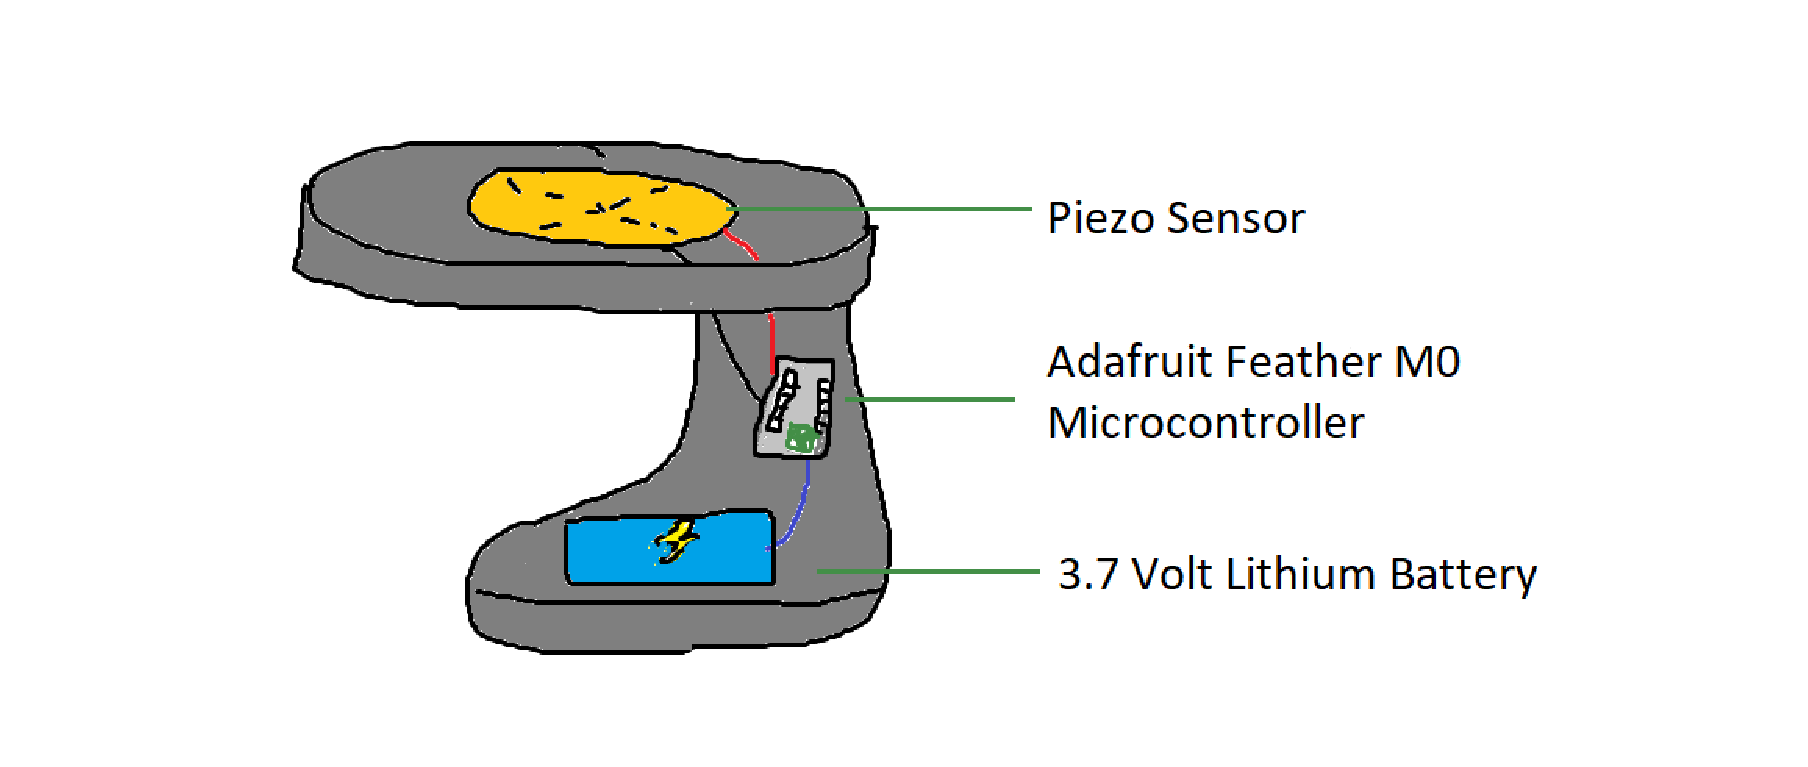
\includegraphics[width=.8\textwidth]{TutTutFirstDraft.eps}
\end{center}

\section{Retrospective}

\begin{center}
\begin{tabular}{ |p{0.3\linewidth}|p{0.3\linewidth}|p{0.3\linewidth}| }
\hline
\multicolumn{3}{|c|}{Retrospective Table} \\
\hline
Positives & Deltas & Actions \\
\hline
Team met semi-often and meetings were effective. & 
Frequency of meetings needs to be increased. & 
We will schedule at least two meetings a week. \\
 & & \\
Team communication was frequent through texting. & 
Another communication medium needs to be explored to improve our accessibility to each other. & 
We will create a Discord server so that we can communicate using our phones and our computers. \\
 & & \\
Each team member participated in writing assignments. & 
Writing assignments need to be started multiple days prior to the due date. & 
We will look at all writing assignment due dates and plan ahead to start them 2-3 days beforehand so that have enough time to complete them. \\
 & & \\
Our client is on campus. & 
Since our client is very busy, more of an effort needs to made to communicate and schedule meetings with him.  & 
We will use BaseCamp to send him questions and requests. If he does no answer, then we will assign him tasks so that he knows what he needs to do for us.  \\
 & & \\
We have access to the OPEnS Lab on campus to test our sensors and 3D Print components. & 
We require weekend or after-hour access in order effectively complete our project. & 
We will talk with our client to work out ways we can have more access to the OPEnS Lab.  \\
 & & \\
All of the parts and components we need to complete the project are in our possession. & 
We will utilize the parts to start sensing vibrations and displaying data. & 
We will connect the sensors to the microcontroller and use code to detect taps on the sensors. We will then start testing it with water and pipettes. \\
 & & \\
\hline
\end{tabular}
\end{center}

\pagebreak

\bibliography{reference}
\bibliographystyle{ieeetr}

\end{document}
